\documentclass[twocolumn]{article}

%\usepackage[iso]{umlaute}
%\usepackage{german}
\usepackage{graphicx}
\usepackage{listings}
\usepackage{amsmath,amssymb,amsthm}
%\usepackage[left=1in,right=1in,top=1in,bottom=1in]{geometry}
\setlength{\parindent}{0cm}
\setlength{\columnsep}{25pt}
\sloppy
\setlength\parindent{24pt}
\newcommand{\lambdaLVar}{\ensuremath{\lambda_{\textrm{LVar}}}}
\newcommand{\userleq}{\ensuremath{\sqsubseteq}}
\newcommand{\Loc}{\mathit{Loc}}
\newcommand{\fmap}{\ensuremath{\stackrel{\textrm{fin}}{\rightarrow}}}
\newcommand{\setof}[1]{\left\{#1\right\}}
\newcommand{\topS}{\ensuremath{\top\hspace{-0.85mm}_{S}}}
\newcommand{\leqstore}[2]{\ensuremath{#1 \userleq_S #2}}
\newcommand{\LVarsDefStore}{
\begin{definition}[store, $\lambdaLVar$]\label{def:lvars-store}
A \emph{store} is either a finite partial mapping $S : \Loc \fmap (D
- \setof{\top})$, or the distinguished element $\topS$.
\end{definition}}
\newcommand{\dom}[1]{\ensuremath{\mathit{dom}(#1)}}
\newcommand{\lubstore}[2]{\ensuremath{#1 \sqcup_{S} #2}}
\newcommand{\userlub}[2]{\ensuremath{#1 \sqcup #2}}

% Your name
\author{Nishanth Nagendra \\ Technische Universit\"at M\"unchen}

\title{Seminar: Programming models and Code Generation\\
       Winter Term 2014/2015\\
       {\bf Quasi deterministic parallel programming using LVars}
}

% Date of your talk
\date{15.01.2015}


\begin{document}

\maketitle

\begin{abstract}
A \textit{deterministic program} always produces the same observable result on multiple runs and a \textit{deterministic by construction parallel programming model} allows only such programs to be written offering programmers freedom from hard to reproduce non deterministic bugs. This report talks about \textit{Lvish}, a \textit{quasi deterministic parallel programming model} that extends \textit{LVars}, its predecessor, which is a deterministic model. LVars generalize existing single assignment models by allowing communication through shared monotonic data structures with monotonic write operations and threshold read operations that block until a lower bound is reached. The semantics are defined in terms of an application specified lattice. LVish extends LVar by allowing to freeze them in order to read their exact contents and to attach event handlers to an LVar triggering a callback when their state changes. It offers quasi determinism in the worst case which means on every run it either produces the same result or raises an error. The LVish model yields promising parallel speedup on benchmarking applications using a prototype implementation of a library in haskell.
\end{abstract}

% \section defines numbered parts of the paper with titles
% there also are \subsection and \subsubsection
\section{Introduction}

% Use labels to be able to refer to this position from somewhere else
\label{introduction}

The purpose of a deterministic-by-construction programming model is to rule out programs like the following from being written, or force them to behave deterministically.  Written in a hypothetical parallel language. 
\begin{lstlisting}
let _ = put lv 3 in  /write 3 in lv/
let par v = get lv  /read from lv/
	_ = put lv 4  /write 4 in lv/
	  in v   /final value is v/
\end{lstlisting}
The \textit{let par} expression, evaluates the two sub-expressions in parallel. The value of $v$ is the value of the entire program. Depending on the scheduler \textit{get} $lv$ or \textit{put} $l 4$ can run first, $v$ might be either $3$ or $4$ during multiple runs giving rise to non determinism.\par
A popular approach for enforcing determinism is to require that variables can only be assigned to once, giving us a single-assignment language. Our program would be invalid because it tries to write to l twice. Single-assignment variables with blocking read semantics, often known as IVars, turn up in all kinds of deterministic parallel systems. But the single-assignment rule disallows a number of programs that we’d like to permit like a program that writes the same value to an IVar twice.
As another example, consider the problem of filling in various parts of a data structure in parallel. Say that l contains a pair, and we’re writing to l twice, with each write filling in one component of the pair. \par 
\begin{lstlisting}
let par  _ = put l (4, )
         _ = put l (, 3) /error/
         in get l
\end{lstlisting}  
Read from l is possible once both writes have completed, so it will always be (4, 3). But single-assignment rules out this program(although we could fake it by using a distinct IVar for each component of the pair, but with more sophisticated data structures it becomes difficult to fake a solution with IVars.)\par

There is a need to generalize the single-assignment model to something that admits programs like these but retains determinism. Deterministic algorithms must be expressible in a style that guarantees determinism, and non-deterministic behaviors, where desired, must be requested explicitly. More generally, enforcing deterministic semantics simplifies composing, porting, reasoning about, debugging, and testing parallel software. Language-level enforcement of determinism is possible, but existing models tend to lack features that would make them applicable to a broader range of problems. Moreover, they lack extensibility: it is difficult to add or change language features without breaking the determinism guarantee. \\ \\
\textit{\textbf{Existing models}} A number of models currently exist as a part of the long running effort towards deterministic by construction parallel programming. \par
\begin{itemize}
        \item \textit{No-shared-state parallelism}: Pure functional programming in Haskell with par and pseq combinators is an example. It uses function level task parallelism or futures. This kind of parallelism does not allow for any shared mutable state between tasks, forcing tasks to produce values independently. Models based on pure data parallelism like \textit{Data parallel Haskell, River Trail API for Java script} also falls in this category,
        \item \textit{Data-flow parallelism}: Kahn process networks, snychronous data flow systems are examples. In these models tasks can only communicate via channels which are FIFO queues where the read operation on these queues is blocking until data is available. Stream-processing languages such as \textit{StreamIt} are based on KPN., 
        \item \textit{Single-assignment parallelism}: IVars are an example which are memory locations that can be either full or empty and can only be assigned once. Reads are blocking for IVars. They have been used in the \textit{monad-par} Haskell library, \textit{Intel CnC(Concurrent collections)}, Concurrent ML(as SnycVars).,
        \item \textit{Imperative-disjoint parallelism}: The state accessed by concurrent threads are disjoint. \textit{Deterministic Parallel Java} falls under this category.     
\end{itemize} 
A common theme that emerges in the study of deterministic-by-construction systems is the notion of monotonicity. Many deterministic parallel programs cannot be expressed with these models. Sharply restricted communication and synchronization capabilities have consequences not only for the immediate usability of guaranteed-deterministic languages, but for those languages’ extensibility as well.
\\ \\ 
\textit{\textbf{Motivating Example}} Consider applications in which independent sub-computations contribute information to shared data structures that are unordered, irregular, or application-specific. An example where issues of ordering create a tension between parallelism and determinism. \par 
In a directed graph where v represents a particular node, we wish to find all (or the first k degrees of) node connected to v, then analyze each node in that set. Existing parallel solutions [1] often use a nondeterministic traversal of the connected component even though the final connected component is deterministic. For example, IVars cannot accumulate sets of visited nodes, nor can they be used as “mark bits” on visited nodes, since they can only be written once and not tested for emptiness. Streams, on the other hand, impose an excessively strict ordering for computing the unordered set of vertex labels in a connected component. A purely functional attempt is given in the original paper[1] where connected-component discovery is parallel, but members of the output set do not become available to other computations until component discovery is finished, limiting parallelism. 
An LVars based programming model can possibly allow us to write a breadth first search traversal where threads communicate using shared monotonic data structures. Consumers of the data structure may execute as soon as data is available, but may only observe irrevocable, monotonic properties of it. 

\section{LVars and LVish}
\subsection{LVars}
An LVar is a memory location that can be shared between multiple threads whose contents can only grow bigger over time, for some definition of “bigger” that the user of the LVar gets to specify. \par
LVars, short for lattice variables, are a generalization of IVars, which are variables that can only be written to once. (The “I” is for “immutable”.) LVars, on the other hand, allow multiple writes, as long as those writes are monotonically increasing with respect to a user-specified lattice. Meanwhile, LVar reads have to specify a threshold set of possible states. A read will block until one of the states in the threshold set has been reached, and then return that state. Information can never be removed and the order in which it is added is not observable. IVars turn out to be a special case of LVars. 
The property of monotonically increasing write operations is enforced by the language. The semantics of put says that a write to a location is the least upper bound of the new value and the current value. 
\begin{lstlisting}
let par _ = put num 3
        _ = put num 2
  in get num /always 3/
\end{lstlisting}
Monotonic writes alone aren't enough to ensure deterministic programs. The above program is non-deterministic where num's notion of “bigger” is “>=”. Despite writes always being monotonically increasing. Get might read either 2 or 3, depending on the order of put/get operations determined by the scheduler. \par
\begin{itemize}
\item To maintain determinism, get operation is restricted: instead of reading the LVar’s exact value, we read one of a set of lower bounds on its value that are given as an extra argument to get. The get operation will block until the LVar reaches a value that is at or above one of those lower bounds. For the above example, the threshold set will just be  {3}. Get operation is called a threshold read, because the value it returns is the threshold we’ve crossed.
\item Once num's value it is at least 3, it will remain at or above 3 forever. As long as we only access them through the put/get interface, LVars are thread-safe: we can safely share them between threads without introducing unintentional non-determinism. That is, puts and gets can happen in any order, without changing the value that a program evaluates to.
\end{itemize}
\begin{center}
\textit{Monotonically increasing writes + threshold reads = deterministic parallelism}
\end{center}
The resulting model is general enough to subsume the existing single-assignment model.
The user-specified set just needs to be a join-semilattice, which is a partially ordered set in which every two elements have a least upper bound. 

To describe Lvar formally, a parallel call-by-value $\lambda$-calculus named $\lambdaLVar$ is introduced in the paper [1] which is extended with a store and communication primitives put and get that operate on data in the store. The definition of $\lambdaLVar$ is parameterized by the choice of lattice and therefore $\lambdaLVar$ is actually a family of languages, rather than a single language. An LVar may have an arbitrary number of states forming a set $D$, which is partially ordered by a relation $\userleq$. Formally, $D$ is a \emph{bounded-join-semilattice} augmented with a greatest element $\top$. 

% free floating figure using width of full page, to be put on [t]op.
%\begin{figure}
%\centerline{
%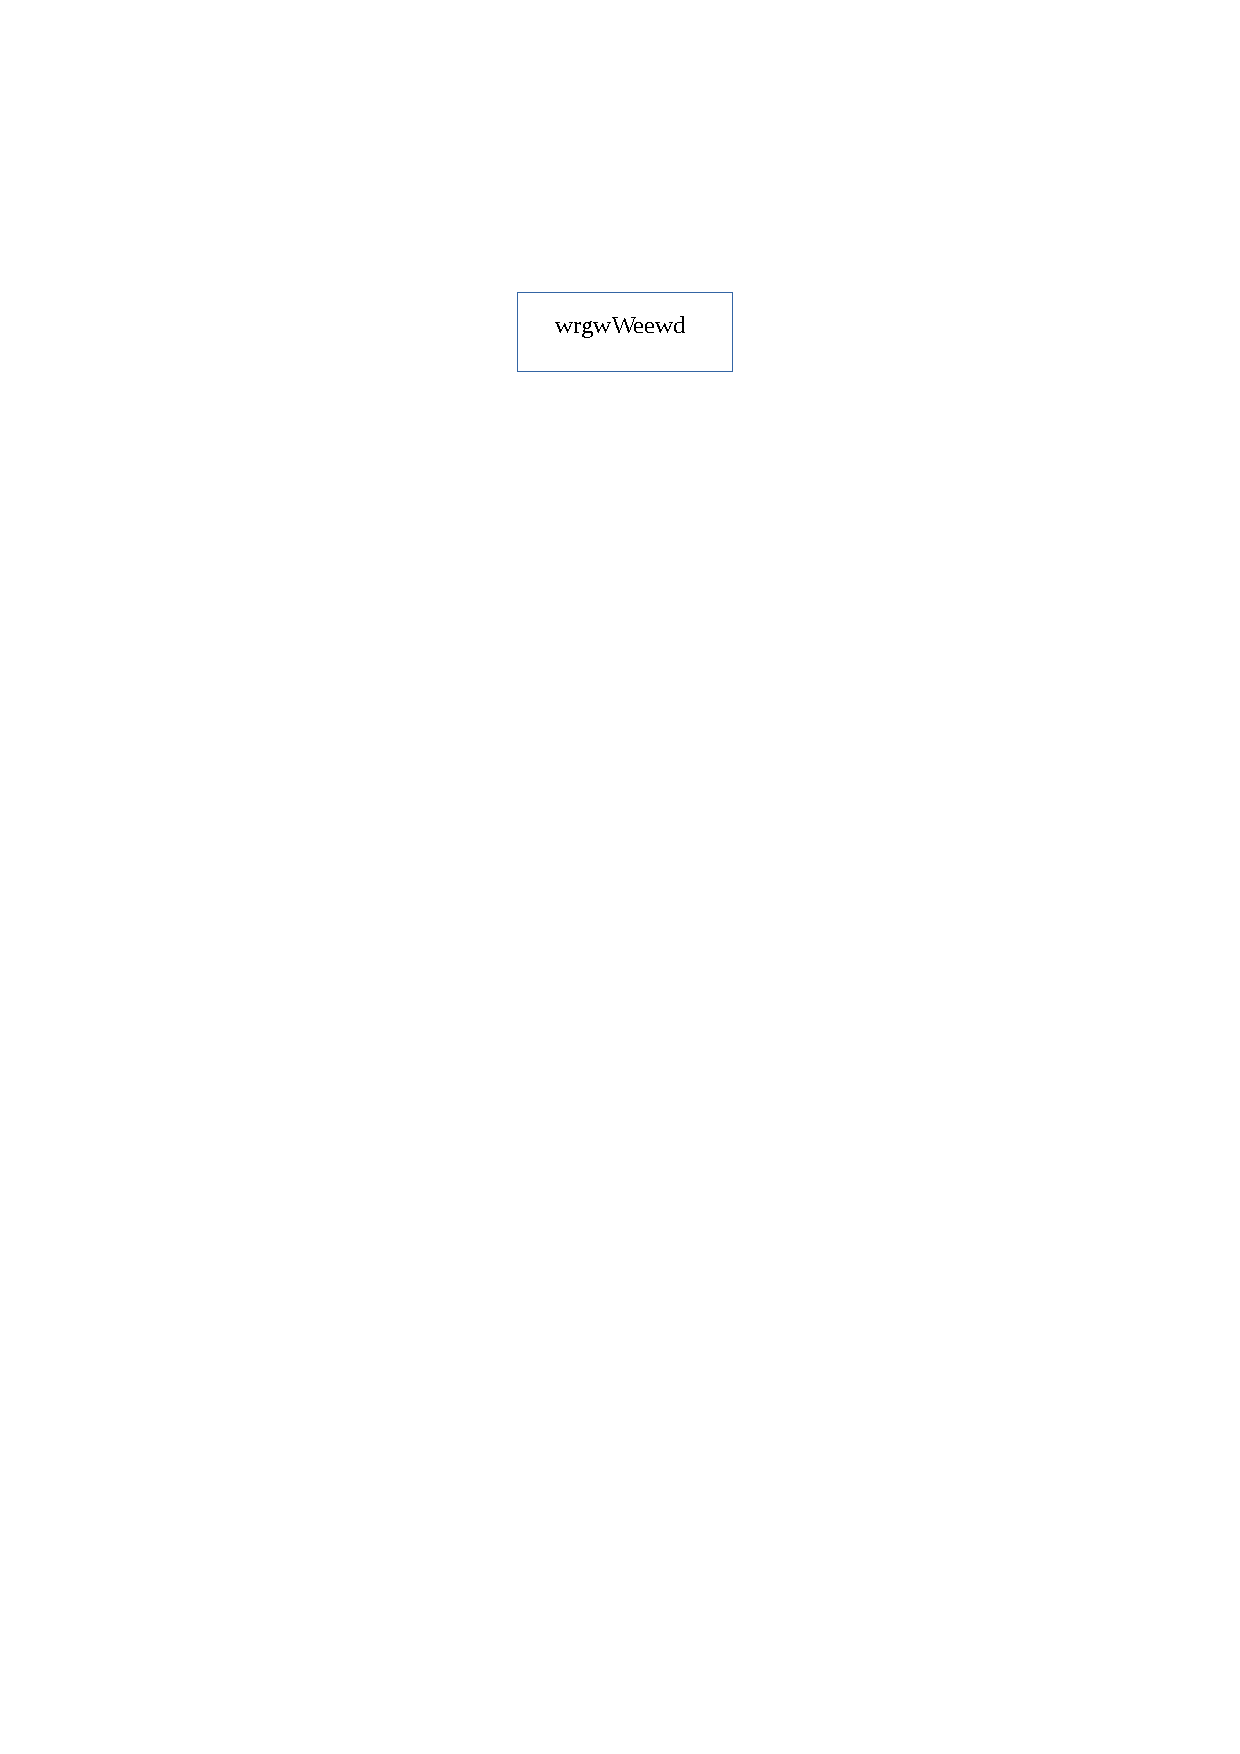
\includegraphics[height=2in,width=1.0\columnwidth]{Figures/try.jpg}
%}
%\caption{A nice caption. The larger width allows for more text without
%taking too much space.}
%\label{Fig2}
%\end{figure}
\begin{itemize}
\item $D$ has a least element $\bot$, representing the initial “empty” state of an Lvar,
\item $D$ has a greatest element $\top$, representing the “error” state that results from conflicting updates to an Lvar,
\item $D$ comes equipped with a partial order $\userleq$, where $\bot \userleq d \userleq \top$ for all $d \in D$.
\item Every pair of elements in $D$ has a least upper bound (lub) written $\sqcup$ which means it is possible for two sub-computations to independently update an LVar, and then deterministically merge the results by taking the lub of the resulting two states.
\end{itemize}
Data structures like arrays, tree, maps , streams etc. can be represented  as lattice. Figure 2 gives three examples of lattices for common data structures.
 
During the evaluation of a $\lambdaLVar$ program, a \emph{store} $S$ keeps track of the states of LVars. Each LVar is represented by a \emph{binding} from a location $l$, drawn from a countable set $\Loc$, to its \emph{state}, which is some element $d \in D$. Although each LVar in a program has its own state, the states of all the LVars are drawn from the same lattice D. We can do this with no loss of generality because lattices corresponding to different types of LVars could always be union ed into a single lattice (with shared $\bot$ and $\top$ Elements). \\ \\
\textbf{Definition 1}: A \emph{store} is either a finite partial mapping $S : \Loc \fmap (D - \setof{\top})$, or the distinguished element $\topS$. \\ \\
The state space of stores forms a \emph{bounded-join-semilattice} augmented with a greatest element, just as $D$ does, with the empty store $\bot_S$ as its least element and $\top_S$ as its greatest element. The $\userleq$ and $\sqcup$ operations defined on elements of $D$ can be lifted to the level of stores.\\ \\
\textbf{Definition 2}: 
 A store $S$ is \emph{less than or equal to} a store $S'$ (written
$\leqstore{S}{S'}$) iff:
\begin{itemize}
\item $S' = \topS$, or
\item $\dom{S} \subseteq \dom{S'}$ and for all $l
\in \dom{S}$, $S(l) \userleq S'(l)$.
\end{itemize}

\textbf{Definition 3}:  The lub of stores $S_1$ and $S_2$ (written $\lubstore{S_1}{S_2}$) is
defined as follows:
\begin{itemize}
\item $\lubstore{S_1}{S_2} = \topS$ iff there exists some $l \in
\dom{S_1} \cap \dom{S_2}$ such that $\userlub{S_1(l)}{S_2(l)} = \top$.
\item Otherwise, $\lubstore{S_1}{S_2}$ is the store $S$ such that:
\begin{itemize}
\item $\dom{S} = \dom{S_1} \cup \dom{S_2}$, and
\item For all $l \in \dom{S}$:
\end{itemize}
\begin{displaymath}
S(l) = \left\{ \begin{array}{ll}
\userlub{S_1(l)}{S_2(l)} & \textrm{if $l \in \dom{S_1} \cap \dom{S_2}$} \\
S_1(l) & \textrm{if $l \notin \dom{S_2}$} \\
S_2(l) & \textrm{if $l \notin \dom{S_1}$}
\end{array} \right.
\end{displaymath}
\end{itemize}
By Definition 3, if d1 t d2 = >, then [l 7! d1] tS [l 7! d2] = >S. Notice that a store containing a binding l 7! > can never arise during the execution of a §LVar program, because an attempted write that would take the state of l to > would raise an error before the write can occur.

3.3 Communication Primitives
The new, put, and get operations create, write to, and read from LVars, respectively. 
¤new extends the store with a binding for a new LVar whose initial state is ?, and returns the location l of that LVar (i.e., a pointer to the LVar).
¤put takes a pointer to an LVar and a singleton set containing a new state and updates the LVar’s state to the least upper bound of the current state and the new state, potentially pushing the state of the LVar upward in the lattice. Any update that would take the state of an LVar to > results in an error.
¤get performs a blocking “threshold” read. It takes a pointer to an Lvar and a threshold set Q, which is a non-empty subset of D that is pairwise incompatible, meaning that the lub of any two distinct elements in Q is >. If the LVar’s state d in the lattice is at or above some d0 2 Q, the get operation unblocks and returns the singleton set fd0g. Note that d0 is a unique element of Q, for if there is another d00 6= d0 in the threshold set such that d00 v d, it would follow that d0 t d00 v d 6= >, which contradicts the requirement that Q be pairwise incompatible.
For Lambda Lvar syntax and semantics, remaining definitions and its details please refer XXX. Lambda Lvar follows parallel reduction semantics [Fork join parallelism]

Proof of determinism: The key to the determinism is the frame rule given below:
XXXXXX
XXXXXxx

A frame property captures the idea of local reasoning about programs that alter state. Written as an inference rule it might look something like this frame rule, due to O’Hearn, Reynolds, and Yang from their work on separation logic: 

XXXXXXXXXX
Here, C is a program, and {p} C {q} is a Hoare triple (in the style of Hoare logic) specifying the behavior of C: it says that if the assertion p  is true before C  runs, then the assertion q  will be true afterwards. For example, p and q  might respectively describe the state of the heap before and after a heap location is updated by C.. Then, the frame rule tells us that running C starting from a state satisfying the assertion p∗r will result in a state satisfying the assertion q∗r. The assertion p∗r is satisfied by a heap if the heap can be split into two non-overlapping parts satisfying p and r, respectively.
In the setting of LVars, the frame property that captures the idea that independent effects commute with each other. Consider an expression e that runs starting in store S  and steps to the expression e′, updating the store to S′. Frame property provides a double-edged guarantee about what will happen if we evaluate e starting from a larger store S⊔R, where R is some other store that we are “framing on” to S, then e  will update the store to S′⊔R, and e will step to e′. Intuitively, the “frame” store R  is a store resulting from some other independently-running computation.1
S and R (or S′ and R) need not be disjoint — we’re combining them with ⊔, not with ∗. If they did have to be disjoint,  — it would mean that concurrent operations cannot touch the same parts of the store. The whole point of LVars is that this kind of total disjointness is unnecessary, since updates commute! Instead, we can behave as though S and R are disjoint, even though they might not be. 
Diamond Lemma
Lemma 4 does the heavy lifting of the determinism proof: it establishes the diamond property, which says that if a configuration steps to two different configurations, there exists a single third configuration to which those configurations both step. 
For supporting lemmas, its details and complete proofs please refer to XXXXXXXXXX. Lemmas there also show  how cases of deadlocks and livelocks are also handled.
The LVars model guarantees determinism by monotonic write operations[which can commute with each other] and threshold read operations. Unfortunately, it is not as general-purpose as one might hope. Consider an unordered graph traversal. A typical implementation involves a monotonically growing set of “seen nodes”; neighbors of seen nodes are fed back into the set until it reaches a fixed point. These are not expressible using the threshold read and least-upper-bound write operations described above. The problem is that these computations rely on negative information about a monotonic data structure, i.e., on the absence of certain writes to the data structure. In a graph traversal, for example, neighboring nodes should only be explored if the current node is not yet in the set; a fixpoint is reached only if no new neighbors are found; and, of course, at the end of the computation it must be possible to learn exactly which nodes were reachable. But in the LVars model, asking whether a node is in a set means waiting until the node is in the set, and it is not clear how to lift this restriction while retaining determinism.
\subsection{LVish}
Lvish extends the Lvars model with 2 additional capabilities. First, it adds event handlers, a mechanism for attaching a callback function to an LVar that runs, asynchronously, whenever events arrive (in the form of monotonic updates to the Lvar). Second, a primitive for freezing an LVar, which comes with the following tradeoff: once an LVar is frozen, any further writes that would change its value instead throw an exception; on the other hand, it becomes possible to discover the exact value of the LVar, learning both positive and negative information about it, without blocking.
Freezing does not commute with writes. If a freeze is interleaved before such a write, the write will raise an exception; if it is interleaved afterwards, the program will proceed normally. Although it appears like determinism is lost, these programs satisfy the property of Quasi determinism that is they will always output the same result or an error.
addHandler lv f1; 3; 5; : : : g (x: put lv x + 1) : registers a handler for lv that executes the callback function x: put lv x + 1 for each odd number that lv is at or above. Event sets are a mathematical modeling tool only; they have no explicit existence in the implementation. Event handlers in LVish invoke their callback for all events in their event set Q that have taken place (i.e., all values in Q less than or equal to the current LVar value), even if those events occurred prior to the handler being registered.
Example program
Can Example 5 ever block? If a callback only executed for events that arrived after its handler was registered, or only for the largest event in its handler set that had occurred, then the example would be nondeterministic: it would block, or not, depending on how the handler registration was interleaved with the puts. By instead executing a handler’s callback once for each and every element in its event set below or at the LVar’s value, we guarantee quasideterminism— and, for Example 5, guarantee the result of 2.

Quiescence through handler pools
Because event handlers are asynchronous, we need a separate mechanism to determine when they have reached a quiescent state, i.e., when all callbacks for the events that have occurred have finished running. Detecting quiescence is crucial for implementing fixpoint computations. To build flexible data-flow networks, it is also helpful to be able to detect quiescence of multiple handlers simultaneously. This design includes handler pools, which are groups of event handlers whose collective quiescence can be tested.
let h = newPool
in addInPool h lv Q f;
quiesce h
The quiesce operation blocks until all of the callbacks running in a particular handler pool, in this case h, are done running. 
where lv is an LVar, Q is an event set, and f is a callback. Handler pools are created with the newPool function, and handlers are registered with addInPool. Whether or not a handler is quiescent is a non-monotonic property: we can move in and out of quiescence as more puts to an LVar occur. There is no risk to quasi-determinism, however, because quiesce does not yield any information about which events have been handled—any such questions must be asked through Lvar functions like get. In practice, quiesce is almost always used together with freezing, which we explain next.
 The freeze operation is a non-blocking read that lets us find out the exact contents of an LVar. We call freeze seen on the last line of our traverse function, and it returns the LVar’s contents.
After freezing, any further writes that would change LVar's state will raise an exception! So it’s good to quiesce before we freeze making it safe to look at the LVar’s exact contents. Aren’t we right back to non-determinism if we forget to quiesce(acts like a synchronization barrier)? For a program that performs freezes, we can guarantee that there are only two possible outcomes: either the deterministic result of all the effects, or a write-after-freeze exception that can assist in debugging the synchronization bug.  We call this property quasi-determinism, and hence the Lvish model is quasi-deterministic; 
The particular graph traversal we saw above is deterministic. In general, freezing introduces quasi-determinism to the programming model, because we might freeze before we’ve quiesced, or because our thread that’s freezing and quiescing might be racing with some other thread to write into a shared LVar.
But, if it is ensured that freezes only ever happen after all writes have completed, then the computations should be deterministic, because then there wouldn’t be any write-after-freeze races. This can be enforced at the implementation level which takes care of quiescing and freezing at the end of a computation. In the LVish library, this is provided by the runParThenFreeze function.

[Paper] contains a core calculus for LVish—in particular, a quasi-deterministic, parallel, call-by-value -calculus extended with a store containing LVars. It extends the original LVar formalism to support event handlers and freezing. The definition of the LVish calculus is parametrized by a single application-specific lattice. Therefore LVish is really a family of calculi, varying by choice of lattice. Rather than modeling the full ensemble of event handlers, handler pools, quiescence, and freezing as separate primitives, it instead formalizes the “freeze-after” pattern—which combined them—directly as a primitive for simplicity.

An LVar’s state is now a pair (d; frz ), where d is an element of the application-specific set D and frz(Short for freeze) is a “status bit” of either true or false. An ordering vp on LVar states (d; frz ) in terms of the application-specific ordering v on elements of D. Every element of D is “freezable” except >. Informally:  Two unfrozen states are ordered according to the application specific v; that is, (d; false) vp (d0; false) exactly when d v d0.
 Two frozen states do not have an order, unless they are equal:
(d; true) vp (d0; true) exactly when d = d0.
 An unfrozen state (d; false) is less than or equal to a frozen state
(d0; true) exactly when d v d0.
 The only situation in which a frozen state is less than an unfrozen
state is if the unfrozen state is >; that is, (d; true) vp
(d0; false) exactly when d0 = >. The addition of status bits to the application-specific lattice results in a new lattice (Dp;vp;?p;>p), and we write tp for the least upper bound operation that vp induces.

During the evaluation of LVish programs, a store S keeps track of the states of LVars and represents them by a binding from a location l, drawn from a set Loc, to its state, which is some pair (d; frz ) from the set Dp.
For detailed syntax and semantics of Lvish please refer to the paper.

Communication primitives are same as Lvar except that new will now create a binding for a new Lvar whose initial state is (I, flase). Put takes a pointer to the Lvar and a new lattice element which is a pair. Get similarly takes a threshold set containing pairs.
Freeze-after-with  primitive: freeze elv after eevents with ecb has the following semantics: It attaches the callback ecb to the LVar elv. The expression eevents must evaluate to a event set Q; the callback will be executed, once, for each lattice element in Q that the LVar’s state reaches or surpasses. The callback ecb is a function that takes a lattice element as its argument. Its return value is ignored, so it runs solely for effect. For instance, a callback might itself do a put to the LVar to which it is attached, triggering yet more callbacks. If the handler reaches a quiescent state, the LVar elv is frozen, and its exact state is returned (rather than an under-approximation of the state, as with get).

To keep track of the running callbacks, LVish includes an auxiliary form,
freeze l after Q with x: e0; fe; : : : g ;H
where:
 The value x: e0 is the callback function;
 The set of expressions fe; : : : g are the running callbacks; and
 The set H represents those values in Q for which callbacks have already been launched.
detects quiescence by checking: First, every event of interest that has occurred (is bounded by the current LVar state) must be handled (be in H). Second, all existing callback threads must have completed and terminated with a value. When such a quiescent state is detected LVar’s state is freezed.  Therefore, freezing is a way of “betting” after quiescence, that no further puts that change the Lvar’s value will occur. To ensure this, we need to guarantee that quiescence is a permanent state, rather than a transient one In practice, freezing is usually the very last step of an algorithm, permitting its result to be extracted. The runParThenFreeze function present in the library does this, and thereby guarantees full determinism.

Proof of Quasi determinism for Lvish: Our main result, Theorem 1, says that if two executions starting from a configuration  terminate in configurations 0 and 00, then 0 and 00 are the same configuration, or one of them is error.
Theorem 1 (Quasi-Determinism). If  ,! 0 and  ,! 00, and neither 0 nor 00 can take a step, then either:0 = 00 up to a permutation Similar to Lvars, it uses the frame property given below by a lemma called independence lemma. 
Lemma 3 (Independence). If hS; ei ,! hS0; e0i (where hS0; e0i 6= error), then we have that: hS tS S00; ei ,! hS0 tS S00; e0i,
where S00 is any store meeting the following conditions:
 S00 is non-conflicting with hS; ei ,! hS0; e0i,
Lemma 3 requires as a precondition that the stores S0 tS S00 and S are equal in status—that, for all the locations shared between them, the status bits of those locations agree. This assumption rules out interference from freezing. Finally, the store S00 must be non-conflicting with the original transition from hS; ei to hS0; e0i, meaning that locations in S00 cannot share names with locations newly allocated during the transition; this rules out location name conflicts caused by allocation. 
Definition 4. Two stores S and S0 are equal in status (written
S =frz S0) iff for all l 2 (dom(S) \ dom(S0)),
if S(l) = (d; frz ) and S0(l) = (d0; frz 0), then frz = frz 0.
Definition 5. A store S00 is non-conflicting with the transition
hS; ei ,! hS0; e0i iff (dom(S0)  dom(S)) \ dom(S00) = ;.
\section{Implementation and Performance}
A prototype implementation of Lvish is available as a monadic library in Haskell, which is available at:
XXXXXXXXXXXXXXXX
It adopts the basic approach of the par monad. The existing Par monad in Haskell offers an API for parallel programming.  It works for parallelizing both pure and IO computations, although only the pure version is deterministic. It provides a work-stealing scheduler that divides the work as evenly as possible between the available processors at runtime. and supports forking tasks that are much lighter weight than IO-threads. As it is implemented as a library, aspects of its behavior can be changed without effecting the compiler or the runtime system. Par can be used for specifying pure parallel computations in which the order of the computation is not known beforehand. The programmer specifies how information flows from one part of the computation to another, but not the order in which computations will be evaluated at runtime. Information flow is described using IVars, which support put and get operations.  The par model does not combine parallelism with lazy evaluation. so sharing and granulairty are completely under the control of the programmer. New units of parallel work are only created by fork and a few other combinators. With LVish we get a lattice-generic infrastructure: the Par monad itself, a thread scheduler, support for blocking and signaling threads, handler pools, and event handlers. Since this infrastructure does not guarantee quasideterminism, only data structure authors should import it who will implement a specific monotonic data structure using this library providing efficient parallel access, subsequently exporting a limited interface for users of the same thereby ensuring quasi-determinism guarantee. The library provides its own custom scheduler and its programs run only inside their par monad allowing only Lvish-sanctioned side effects to provide compile time guarantees of determinism and quasi determinism.

In order to specify the type of the par computation it provides a phantom type that indicates their determinism level.

Par type constructor:


following suite of run functions
X
Y
Z
If the Lvish code uses freeze then it is marked as QuasiDet or Det if it is fully deterministic. RunparIO allows us to execute Lvish code in the IO monad if the determinism level is arbitrary. RunparthenFreeze automatically freezes the Lvar when it returns back its exact value guaranteeing determinism.
Two key ideas that are inherent to this prototype are atoms and idempotence. Atoms are elements not equal to bottom but whose only smaller element is bottom. Lattices for which every element is the lub of some set of atoms are called atomistic, and most application-specific lattices used by LVish programs have this property—especially those whose elements represent collections. For an atomistic lattice, the corresponding data structure usually exposes operations that work at the atom level, semantically limiting puts to atoms, gets to threshold sets of atoms, and event sets to sets of atoms.     by associating LVars with a set of deltas (changes), as well as a lattice. For atomistic lattices, the deltas are essentially just the atoms—for a set lattice, a delta is an element; for a map, a key/value pair. Deltas provide a compact way to represent a change to the lattice, allowing us to easily and efficiently communicate such changes between puts and gets/handlers.  

idempotence, meaning that dtd = d for any element d. In LVish terms, repeated puts or freezes have no effect,   if the scheduler is allowed to occasionally duplicate work, it is possible to substantially save on synchronization costs. Since LVish computations are guaranteed to be idempotent, we could use such a scheduler (for now we use the standard Chase-Lev deque [10]). But idempotence also helps us deal with races between put and get/addHandler, 
Representation: data LVars, data status, put, remove, listener, etc 
Internally par monad represents computations in continuation passing style, in terms of their interpretation in the IO monad. 
Signature and type of the following methods along with short explanation:
GetLV
putLV
freezeLV
Handler pools and quiescence

An example to illustrate the use of Lvish library is performing a parallel graph traversal given a starting node and finding all the nodes reachable from it. We first create a new LVar of a set type, called seen. Then we attach an event handler to the seen set. The newHandler function, defined elsewhere, takes 2 arguments, first is the LVar, seen, and second is the callback that we want to run every time an event arrives — that is, every time a new node is added to the set. The callback takes that newly arrived node node as its argument, looks up node’s neighbors in the graph by calling a function neighbors (also defined elsewhere), and then maps the insert function over the list of neighbor nodes that neighbors returns. Then, we add the starting node to the seen set with insert startNode seen and the event handler does the rest.
LVar operations can only run inside Par computations which are executed with one of the “run” functions.  runParThenFreeze, executes a Par computation and then returns a frozen LVar at the end of it, after an implicit global barrier. So, if we have a Par computation that side-effects an LVar and we run it with runParThenFreeze, then we don’t have to manually freeze the LVar ourselves, which means we don’t have to manually quiesce, either! 
This function returns a computation of type Par Det, for “deterministic”. The “Det” is an effect level, meaning that the computation can only perform deterministic operations — in particular, it’s not allowed to do a freeze, and if it tried to, then that would be a static type error. If we had called quiesce and freeze explicitly in our code within traverse function, then it would return a computation of type Par QuasiDet, for “quasi-deterministic”. 
traverse starts off the computation and then returns the seen LVar. The LVar may well still be growing at the time traverse returns — but, since runParThenFreeze cannot return unless all threads launched inside the Par computation are done, there’s no threat to determinism, and we’ll always get the same set of nodes as our answer. More generally, the fact that it’s possible to safely return an LVar while it is still being written to by a handler makes it possible to set up dataflow-style, pipeline-parallel networks of LVars, letting us combine task parallelism and pipeline parallelism in the same deterministic program.  

\section{Summary}
\label{summary}

The summary shortly repeats the core ideas and results from the
previous text. If the reader has problems understanding the summary
he knows that he should go back to the relevant sections.
Thus, the last section should consist of:

\begin{itemize}
	\item a summary,
	\item an evaluation of what was done, importance of this work,
	\item what is left, what still needs to be done,
        \item short outlook into the future.
\end{itemize}

Last but not least, we can explain anything missing yet in the evaluation
done in this paper. This allows to refer to what readers can expect from
authors in the future.

% Put citations from bibtex into References section which were not
% explicity cited.
\nocite{robotron,
stonx,vice,650sim,herculessim,zib,4004,thermal1,thermal2,rojas,neumann,
neumann1void,neumann2void,neumann3,neumann4,Siewiorek,AmBlBr,Blaauw:1997:CAC,ChPB97,Brom98,Clym93,Buhu99,
Edwa01,Nill99,ABC+90,Rama91,Heid97,Kist95,Klot03,LMcCL92,LFS+92,LMDD92,Vlec03,Cray77,top500,650,Amda67,
Arla88,ODLD86,Hick04,Walk04}


\bibliographystyle{plain}
% Literature sources are to be found in seminarpaper.bib
\bibliography{seminarpaper} 
\end{document}
